\chapter{Variational Bayesian Approximation
for Medical Diagnosis}
\label{ch-var-bay-medical}

This chapter is based
on Ref.\cite{jaak-jordan}.

A Variational Bayesian Approximation (VBA)
is when we approximate
a probability distribution
by another 
probability distribution that depends
on a continuous ``variational parameter". 
This parameter is
adjusted 
within its range of possible values,
to make the approximation
as good as possible.
There are many VBA methods.
VBA methods are inspired by 
ancient  methods
used in Calculus 
of Variations applied to Physics
and Engineering problems.

In this chapter,
we do VBA  via
Jensen's inequality and
dual functions.

Ref.\cite{jaak-jordan}, on which
this chapter is based,
applies VBA methods to the problem of diagnostic inference using the Quick Medical Reference (QMR) bipartite Bayesian Network. 
According to Ref.\cite{jaak-jordan} 
the maximal clique size of the QMR 
bnet is
150 nodes, which rules out exact methods
of inference like the Junction Tree Algorithm
(see Chapter \ref{ch-junc-tree}).
For such high complexity cases,
one is forced to use
either a VBA or a Monte Carlo method.

\begin{figure}[h!]
$$\xymatrix{
\ul{\ell}
\ar[dr]\ar[drr]\ar[drrr]\ar[drrrr]\ar[drrrrr]
&
&\rvd_1\ar[dl]\ar[drr]
&\rvd_2\ar[dll]\ar[dl]\ar[dr]\ar[d]\ar[drr]
&\rvd_3\ar[dll]\ar[d]\ar[dr]
\\
&\rvs_1
&\rvs_2
&\rvs_3
&\rvs_4
&\rvs_5
}$$
\caption{
Typical bnet (bipartite, 2 level graph) 
for medical diagnosis
to which we will apply VBA
methods.
In this case, $nd=3$ and
$ns=5$. 
According to Ref.\cite{jaak-jordan},
for QMR, $nd\approx 600$ 
and $ns\approx 4000$.
}
\label{fig-var-bay-med-bnet}
\end{figure}

Fig.\ref{fig-var-bay-med-bnet}
gives a typical bnet
for medical diagnosis
to which we will apply VBA methods.
$\rvd_i\in \bool$
for $i=1,2, \ldots, nd$
are the possible diseases,
$\rvs_\s\in\bool$ 
for $\s=1,2, \ldots, ns$ are the possible
symptoms, and $\ul{\ell}\in\bool$
is the leakage  due to 
possible error in 
the parents of the symptoms.
Note that the 
arrows point from
diseases to symptoms
because diseases precede
in time
the symptoms.

Let
\beq
\ZZ_{[1,n]}=\{1,2, \ldots, n\}
\eeq

\beq
pa_\s = \{i\in\ZZ_{[1,nd]}: \rvd_i\in pa(\rvs_\s)\} = \text{ parents of $\rvs_\s$}
\eeq
Note that $pa_\s$
does not include $\ul{\ell}$,
which is also a  parent
of $\rvs_\s$.

\beq
ch_i= \{\s\in\ZZ_{[1,ns]}:
 \rvs_\s\in ch(\rvd_i)\}=
 \text{ children of $\rvd_i$ }
\eeq

\beq
\rvd_{A} =\{\rvd_k: k\in A\}
\eeq

\newcommand{\dall}[0]{d^{nd}}
\beq
\rvd^{nd} =\{\rvd_k: k\in \ZZ_{[1, nd]}\}
\eeq

\beq
\rvd_{!j} =\{\rvd_k: k\in \ZZ_{[1, nd]}-\{j\}\}
\eeq

The TPMs, printed in blue,
for the bnet 
Fig.\ref{fig-var-bay-med-bnet},
are as follows:

\beq \color{blue}
P(d_j) = \text{ given }
\eeq

\beq \color{blue}
P(\ell) = \text{ given }
\eeq

\beqa \color{blue}
P(\rvs_\s=0|d_{pa_\s}, \ell)
&=&\color{blue}
\underbrace{P(\rvs_\s=0|\ell)}_{e^{-\theta_{\s|0}}}
\prod_{j\in pa_\s}
\underbrace{P(\rvs_\s=0|d_j)}_
{e^{-\theta_{\s|j}d_j}}
\\
&=&\color{blue}
e^{-\theta_{\s|0} -
\sum_{j\in pa_\s}\theta_{\s|j}d_j}
\eeqa
where $\theta_{\s|0}, \theta_{\s|j}>0$.
This  
$P(\rvs_\s=0|d_{pa_\s}, \ell)$
corresponds to
the noisy-or model 
(See Chapter \ref{ch-noisy-or}.).

\beq \color{blue}
P(\rvs_\s=1|d_{pa_\s})=
1-
e^{-\theta_{\s|0} -
\sum_{j\in pa_\s}\theta_{\s|j}d_j}
\eeq

Define
\beq
x_\s=
\theta_{\s|0} +
\sum_{j\in pa_\s}\theta_{\s|j}d_j
\eeq
Suppose $A \subset 
\ZZ_{[1,ns]}$, $A^c=\ZZ_{[1,ns]}-A$.
Then

\begin{align}
P(d_j|\rvs_A=0, \rvs_{A^c}=1)&=
 \frac{P(\rvs_A=0, \rvs_{A^c}=1|d_j)P(d_j)}
 {P(\rvs_A=0, \rvs_{A^c}=1)}
 \\
 &=\caln(!d_j)
 \sum_{d_{!j}}P(\rvs_A=0, \rvs_{A^c}=1|\dall)P(\dall)
 \\
 &=\caln(!d_j)
  \sum_{d_{!j}}P(\rvs_{A^c}=1|\dall)
  P(\rvs_A=0|\dall)P(\dall)
\\
&=\caln(!d_j)\sum_{d_{!j}}
\left\{
\begin{array}{l}
\prod_{\s\in A^c}
\overbrace{(1-e^{-x_\s})
}^{\text{ call } \calp_\s}
\\
\prod_{\s\in A}
e^{-\theta_{\s|0}}
\prod_{j\in pa_\s}[e^{-\theta_{\s|j}}]^{d_j}
\\
\prod_{j\in \ZZ_{[1,nd]}} P(d_j)
\end{array}
\right.
\end{align}
Summing
over $d_{!j}$ seems
crazy, because $nd>>1$,
but
we will
approximate
the summand
so that the sum
can be done in closed form.

Define
\beq
f(x_\s)=\ln(1-e^{-x_\s})
\eeq
and

\beq
\calp_\s = 1-e^{-x_\s} = e^{f(x_\s)}
\eeq
$f(x_\s)$
is a concave function.
See Fig.\ref{fig-dual-dual-ln-1-e-x}
for a plot of it.

Next, we
shall find a lower
and upper bound 
for $\calp_\s$.

To find
the upper bound, we will use 
dual functions, which are
discussed in Section
\ref{sec-dual-fun}.

Let $F(X_\s)$ be the dual
 function of $f(x_\s)
 = \ln(1-e^{-x_\s})$).
 In Section
 \ref{sec-dual-fun}, we show that
 
 \beqa
 F(X_\s)&=&
 \min_{x_\s}(x_\s X_\s - f(x_\s))
 \\
 &=&
 -X_\s\ln  X_\s
 +(1+X_\s)\ln(1+X_\s)
 \eeqa
 and

\beq
f(x_\s)\leq x_\s X_\s - F(X_\s)
\;.
\eeq
Therefore



\beqa
\calp_\s
&=&
e^{f(x_\s)}
\\
&\leq &
 e^{x_\s X_\s - F(X_\s)}
 \\
 &=&
 \underbrace{
 e^{-F(X_\s)}
 e^{-\theta_{\s|0}X_\s}
 \prod_{j\in
  pa_\s}[e^{-\theta_{\s|j}X_\s}]^{d_j}
  }_{\text{ call } \calb(X_\s)
  }
\eeqa

To find
a lower bound for $P_\s$,
we will use
Jensen's inequality, which
is discussed in Section
[\nameref{sec-jensens}].
Let $q_{j|\s}\in [0,1]$ 
satisfy $\sum_j q_{j|\s}=1$.
Then


\beqa
\calp_\s &=&
 e^{f(x_\s)}
 \\
 &=&
  e^{f\left(\theta_{\s|0} +\sum_j
 \theta_{\s|j}d_j \right)}
 \\
  &=&
  e^{
  f\left(
  \theta_{\s|0}
  +
  \sum_j q_{j|\s}\frac{\theta_{\s|j}d_j}{q_{j|\s}}
  \right)
  }
 \\
 &\geq&
 e^{
 \sum_j q_{j|\s}
 f\left(
 \theta_{\s|0}
 +\frac{\theta_{\s|j}d_j}{q_{j|\s}}
 \right)
 }
 \\
 &=&
 e^{
 \sum_j
 q_{j|\s}\left[
 d_j f\left(
 \theta_{\s|0} + 
 \frac{\theta_{\s|j}d_j}{q_{j|\s}}
 \right)
 +(1-d_j)f(\theta_{\s|0})
 \right]
 }
 \\
 &=&
 \underbrace{
e^{
f(\theta_{\s|0})+
\sum_j
 q_{j|\s} d_j\left[
  f\left(
 \theta_{\s|0} + 
 \frac{\theta_{\s|j}d_j}{q_{j|\s}}
 \right)
 - f(\theta_{\s|0})
 \right]
 }
 }_{
 \text{ call } \cala(q_{.|\s})
 }
  \eeqa
  
 In conclusion, 
\beq
\boxed{
\cala(q_{.|\s})
\leq
\calp_\s
\leq
\calb(X_\s)
}
\eeq
with 
variational
parameters 
$q_{.|\s}$ and $X_\s$.


\section{Dual Functions}
\label{sec-dual-fun}

\begin{figure}[h!]
\centering
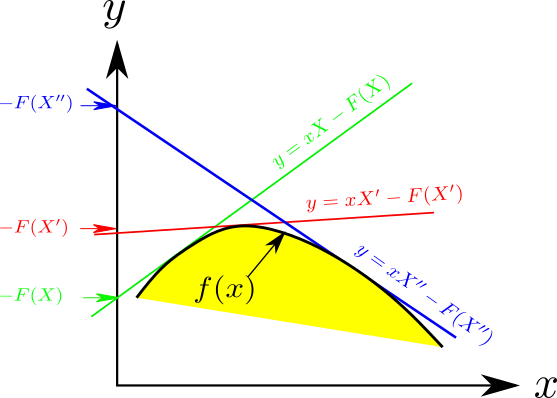
\includegraphics[width=4in]
{var-bay-medical/dual-fun.png}
\caption{The dual
function $f(x)$ of a concave function
$F(X)$
is the osculating (kissing)
locus of the 
family
of lines $y=Xx - F(X)$
for all $X$.}
\label{fig-dual-fun}
\end{figure}


If $f(x)$ is a concave function, we
define its {\bf dual function} by

\beq
F(X) = \min_x (X^T x - f(x))
\label{eq-FX-def}
\;.
\eeq
\begin{claim}
If $f(x)$ is a concave function
with dual $F(X)$, then
\beq
f(x)= \min_X(X^T x - F(X))
\label{eq-fx-as-min}
\eeq

 \beq
 \nabla_X F(X(x)) = (\nabla_x f)^{-1}(x)
 \eeq
Eqs.(\ref{eq-FX-def})  
and (\ref{eq-fx-as-min}) 
are also true if we replace the 
words ``concave" with ``convex"
and ``min" with ``max".
\end{claim}
\proof

Let $x^*$ 
be the value of $x$
which minimizes $F(X)=X^T x-f(x)$
with respect to $x$. Hence,
\beq
F(X) = X^Tx^* - f(x^*)
\;.
\label{eq-FX}
\eeq
Rearranging terms in Eq.(\ref{eq-FX}),
we get

\beq
f(x^*) = X^Tx^* - F(X)
\label{eq-relabel-1}
\eeq

Let $X^*$ 
be the value of $X$
which minimizes $f(x)=X^T x-F(X)$
with respect to $X$. Hence,
\beq
f(x) = (X^*)^Tx - F(X^*)
\label{eq-relabel-2}
\eeq
Replacing $X^*$ by $X$
and $x$ by $x^*$
in Eq.(\ref{eq-relabel-2})
yield Eq.(\ref{eq-relabel-1}).


Note that minimization
with respect to $x$
is achieved if
\beq
X_i = \partial_{x_i}f(x),\;
X = \nabla_x f(x)
\eeq
whereas minimization 
with respect to $X$
is achieved if 

\beq
x_i = \partial_{X_i}F(X),\;x = \nabla_X F(X)
\eeq
Hence,

\beq
x = \nabla_X F(\nabla_x f(x))
\eeq

\qed

See Fig.\ref{fig-dual-fun}
for a geometrical
representation
of Eq.(\ref{eq-fx-as-min}).

We end this section
on dual functions with some
examples.
\hrule
\begin{enumerate}
\item
Find the dual function of
\beq
\boxed{f(x) = e^x}
\;.
\eeq

\beqa
X &=& \partial_{x^*}f
\\
&=&
e^{x^*}
\eeqa

\beq
x^* = \ln  X
\eeq

\beq
f(x^*) = X
\eeq

\beqa
F(X)&=&x^*X - f(x^*)
\\
&=&
X\ln X -X
\eeqa



\hrule
\item 
Find the dual function of
\beq
\boxed{f(x) = f + f'x +\frac{1}{2}f''x^2}
\;.
\eeq

\beqa
X&=&
\partial_{x^*} f
\\
&=&
f' + f''x^*
\label{eq-X-xstar}
\eeqa

\beq
x^* = \frac{X-f'}{f''}
\eeq
\beqa
f(x^*)&=& f
+
f' 
\left[
\frac{X-f'}{f''}\right]
+
\frac{1}{2}f''
\left[\frac{X-f'}{f''}\right]^2
\\
&=&
\left[f - \frac{(f')^2}{2f''}\right]
+
X^2\left[
\frac{1}{2f''}
\right]
\eeqa

\beqa
F(X)&=&
Xx^*-f(x^*)
\\
&=&
X\left[\frac{X-f'}{f''}\right]
-f(x^*)
\\
&=&
\left[-f + \frac{(f')^2}{2f''}\right]
+
X\left[
\frac{-f'}{f''}
\right]
+
X^2\left[
\frac{1}{2f''}
\right]
\eeqa

Note that when $f=f'=0$,
we get 

\beq
f(x)=\frac{f'' x^2}{2} 
,\quad 
F(X)= \frac{X^2}{2 f'' }
\eeq

%\beqa
%x &=&
%\partial_{X^*} F
%\\
%&=& 
%\left[
%\frac{-f'}{f''}
%\right]
%+
%X^*\left[
%\frac{1}{f''}
%\right]
%\eeqa
%
%\beq
%X^* = f' + f''x
%\quad\text{(see Eq.(\ref{eq-X-xstar}))}
%\eeq
%
%\beqa
%F(X^*)&=&
%\left[-f + \frac{(f')^2}{2f''}\right]
%+
%[f' + xf'']
%\left[
%\frac{-f'}{f''}
%\right]
%+
%[f'+f''x]^2
%\left[
%\frac{1}{2f''}
%\right]
%\\
%&=&
%-f + \frac{f''}{2} x^2
%\eeqa
%
%
%\beqa
%f(x)&=& X^*x - F(X^*)
%\\
%&=&
%[f'+f'' x]x
%+f-\frac{f''}{2} x^2
%\\
%&=&
%f + f'x+\frac{f''}{2} x^2
%\eeqa

\hrule

\item
Find the dual function of
\beq
\boxed{f(x)= \ln(1-e^{-x})}
\;.
\eeq

\beqa
X
&=&
\partial_{x^*} f(x^*)
\\
&=&
\frac{e^{-x^*}}{1-e^{-x^*}}
\eeqa

\beq
X=(1+X)e^{-x^*}
\eeq
\beq
x^* = \ln\frac{1+X}{X}
\eeq

\beq
f(x^*)=\ln\left(
1 - \frac{X}{1+X}
\right)=-\ln(1+X)
\eeq

\beqa
F(X) &=& X x^* -f(x^*)
\\
&=&
X \ln\frac{1+X}{X}
+\ln(1+X)
\\
&=&
-X\ln  X
+(1+X)\ln(1+X)
\eeqa
\end{enumerate}


\begin{figure}[h!]
\centering
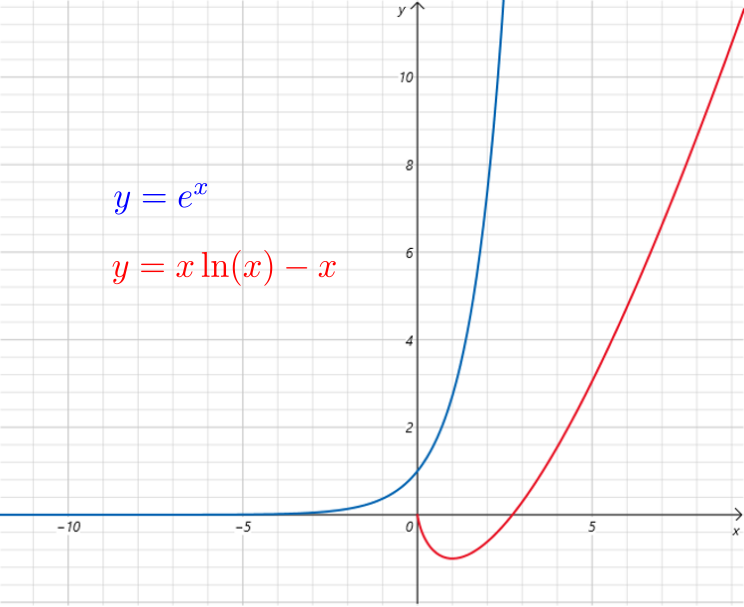
\includegraphics[width=3.5in]
{var-bay-medical/dual-ex.png}
\caption{$f(x)=e^x$ and its dual.}
\label{fig-dual-ex}
\end{figure}

\begin{figure}[h!]
\centering
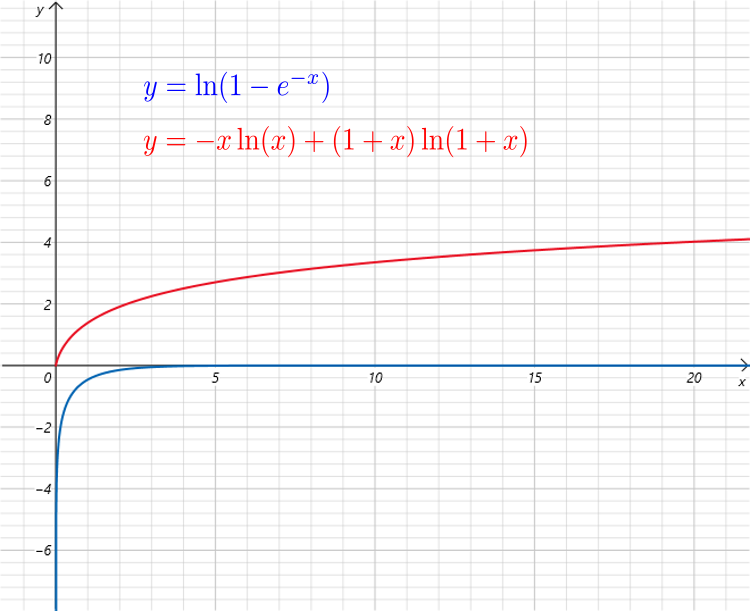
\includegraphics[width=3.5in]
{var-bay-medical/dual-ln-1-e-x.png}
\caption{$f(x)=\ln(1-e^{-x})$ and its dual.}
\label{fig-dual-dual-ln-1-e-x}
\end{figure}



